% A LaTeX template for EXECUTIVE SUMMARY of the MSc Thesis submissions to
% Politecnico di Milano (PoliMi) - School of Industrial and Information Engineering
%
% S. Bonetti, A. Gruttadauria, G. Mescolini, A. Zingaro
% e-mail: template-tesi-ingind@polimi.it
%
% Last Revision: October 2021
%
% Copyright 2021 Politecnico di Milano, Italy. NC-BY

\documentclass[11pt,a4paper,twocolumn]{article}

%------------------------------------------------------------------------------
% REQUIRED PACKAGES AND CONFIGURATIONS
%------------------------------------------------------------------------------
\usepackage{titlesec}
\usepackage{color}

\usepackage[utf8]{inputenc}
\usepackage[english]{babel}
\usepackage[T1]{fontenc}

\usepackage{graphicx}
\graphicspath{{Images/}}
\usepackage{eso-pic}
\usepackage{subfig}
\usepackage{caption}
\usepackage{transparent}

\usepackage{amsmath}
\usepackage{amsthm}
\usepackage{bm}
\usepackage[overload]{empheq}

\usepackage{tabularx}
\usepackage{longtable}
\usepackage{colortbl}
\usepackage{booktabs}

\usepackage{algorithm}
\usepackage{algorithmic}

\usepackage[colorlinks=true,linkcolor=black,anchorcolor=black,citecolor=black,filecolor=black,menucolor=black,runcolor=black,urlcolor=black]{hyperref}
\usepackage{cleveref}
\usepackage[square, numbers, sort&compress]{natbib}
\bibliographystyle{plain}

\usepackage{appendix}
\usepackage{enumitem}

\usepackage{amsthm,thmtools,xcolor}
\usepackage{comment}
\usepackage{fancyhdr}
\usepackage{tcolorbox}
\usepackage{stfloats}

%-------------------------------------------------------------------------
% NEW COMMANDS DEFINED
%-------------------------------------------------------------------------
\newcommand{\bea}{\begin{eqnarray}}
\newcommand{\eea}{\end{eqnarray}}
\newcommand{\e}[1]{\times 10^{#1}}
\newcommand{\mathbbm}[1]{\text{\usefont{U}{bbm}{m}{n}#1}}
\newcommand{\pdev}[2]{\frac{\partial#1}{\partial#2}}

% Define colors used by both the thesis and executive summary templates.
\definecolor{bluepoli}{cmyk}{0.4,0.1,0,0.4}
\definecolor{bluePoli}{cmyk}{0.4,0.1,0,0.4}

\ifdefined\chapter
% Custom theorem environments
\declaretheoremstyle[
  headfont=\color{bluepoli}\normalfont\bfseries,
  bodyfont=\color{black}\normalfont\itshape,
]{colored}

% Set-up caption colors
\captionsetup[figure]{labelfont={color=bluepoli}} % Set colour of the captions
\captionsetup[table]{labelfont={color=bluepoli}} % Set colour of the captions
\captionsetup[algorithm]{labelfont={color=bluepoli}} % Set colour of the captions

\theoremstyle{colored}
\newtheorem{theorem}{Theorem}[chapter]
\newtheorem{proposition}{Proposition}[chapter]

% Enhances the features of the standard "table" and "tabular" environments.
\newcommand\T{\rule{0pt}{2.6ex}}
\newcommand\B{\rule[-1.2ex]{0pt}{0pt}}

% Pseudo-code algorithm descriptions.
\newcounter{algsubstate}
\renewcommand{\thealgsubstate}{\alph{algsubstate}}
\newenvironment{algsubstates}
  {\setcounter{algsubstate}{0}%
   \renewcommand{\STATE}{%
     \stepcounter{algsubstate}%
     \Statex {\small\thealgsubstate:}\space}}
  {}

% New font size
\newcommand\numfontsize{\@setfontsize\Huge{200}{60}}

% Title format: chapter
\titleformat{\chapter}[hang]{
\fontsize{50}{20}\selectfont\bfseries\filright}{\textcolor{bluepoli} \thechapter\hsp\hspace{2mm}\textcolor{bluepoli}{|   }\hsp}{0pt}{\huge\bfseries \textcolor{bluepoli}
}

% Title format: section
\titleformat{\section}
{\color{bluepoli}\normalfont\Large\bfseries}
{\color{bluepoli}\thesection.}{1em}{}

% Title format: subsection
\titleformat{\subsection}
{\color{bluepoli}\normalfont\large\bfseries}
{\color{bluepoli}\thesubsection.}{1em}{}

% Title format: subsubsection
\titleformat{\subsubsection}
{\color{bluepoli}\normalfont\large\bfseries}
{\color{bluepoli}\thesubsubsection.}{1em}{}

% Shortening for setting no horizontal-spacing
\newcommand{\hsp}{\hspace{0pt}}

\makeatletter
% Renewcommand: cleardoublepage including the background pic
\renewcommand*\cleardoublepage{%
  \clearpage\if@twoside\ifodd\c@page\else
  \null
  \AddToShipoutPicture*{\BackgroundPic}
  \thispagestyle{empty}%
  \newpage
  \if@twocolumn\hbox{}\newpage\fi\fi\fi}
\makeatother

%For correctly numbering algorithms
\numberwithin{algorithm}{chapter}

\else
% Executive summary specific setup for article class.
\declaretheoremstyle[
  headfont=\color{bluePoli}\normalfont\bfseries,
  bodyfont=\color{black}\normalfont\itshape,
]{colored}

\captionsetup[figure]{labelfont={color=bluePoli}} % Set colour of the captions
\captionsetup[table]{labelfont={color=bluePoli}} % Set colour of the captions
\captionsetup[algorithm]{labelfont={color=bluePoli}} % Set colour of the captions

\theoremstyle{colored}
\newtheorem{theorem}{Theorem}[section]
\newtheorem{proposition}{Proposition}[section]

\newcommand\T{\rule{0pt}{2.6ex}}
\newcommand\B{\rule[-1.2ex]{0pt}{0pt}}

\newcounter{algsubstate}
\renewcommand{\thealgsubstate}{\alph{algsubstate}}
\newenvironment{algsubstates}{
    \setcounter{algsubstate}{0}%
    \renewcommand{\STATE}{%
    \stepcounter{algsubstate}%
    \Statex {\small\thealgsubstate:}\space}
    }{}

\newcolumntype{L}[1]{>{\raggedright\let\newline\\\arraybackslash\hspace{0pt}}m{#1}}
\newcolumntype{C}[1]{>{\centering\let\newline\\\arraybackslash\hspace{0pt}}m{#1}}
\newcolumntype{R}[1]{>{\raggedleft\let\newline\\\arraybackslash\hspace{0pt}}m{#1}}

\setlist[itemize,1]{label=$\bullet$}
\setlist[itemize,2]{label=$\circ$}
\setlist[itemize,3]{label=$-$}
\setlist{nosep}

\setlength{\columnsep}{30pt}

\newcommand\BackgroundPic{% Adding background picture
	\put(230,358){
		\parbox[b][\paperheight]{\paperwidth}{%
			\vfill
			\centering
			\transparent{0.4}
			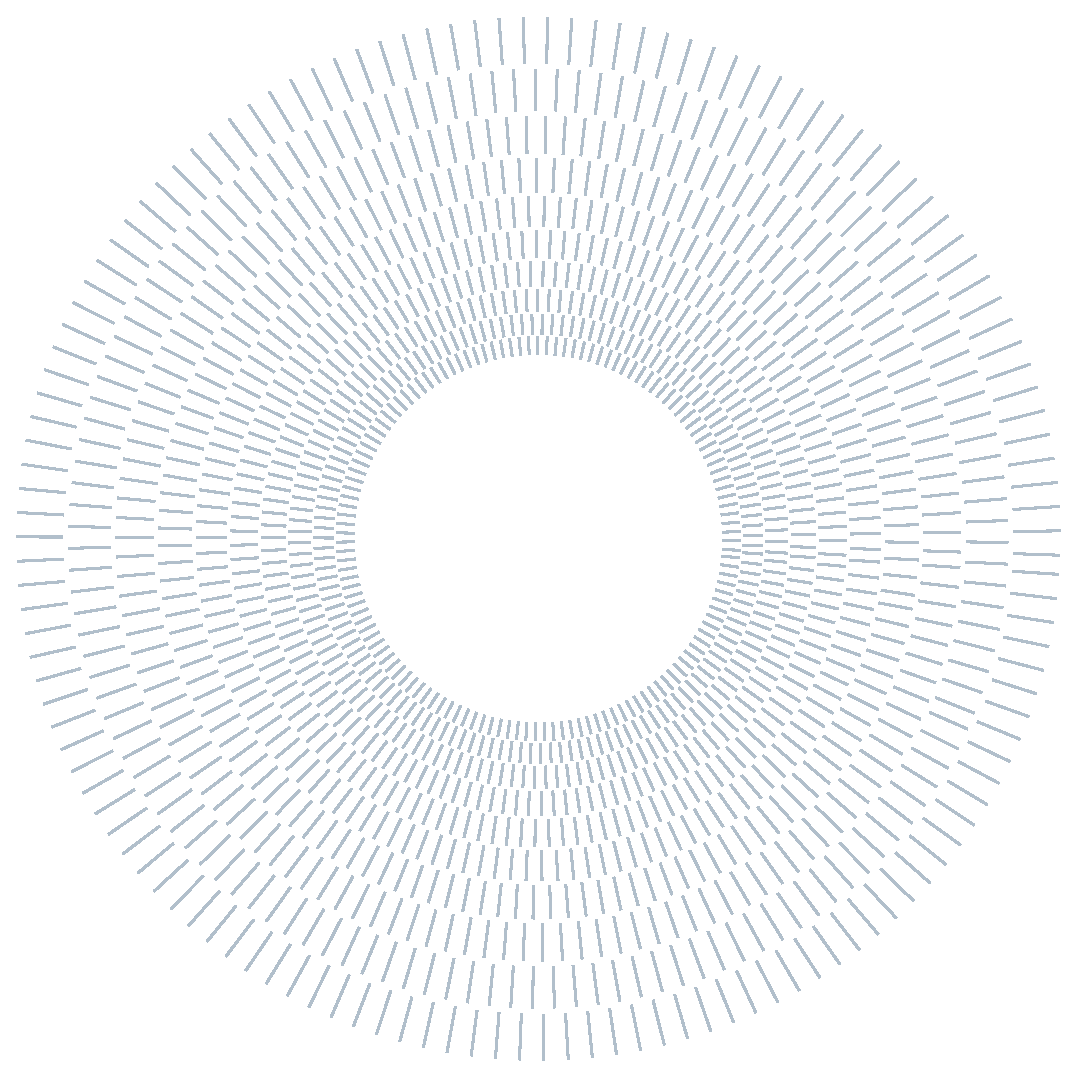
\includegraphics[width=0.5\paperwidth]{raggiera_polimi.eps}%
			\vfill
}}}

\setlength\parindent{0pt}

\titleformat{\section}
{\color{bluePoli}\normalfont\Large\bfseries}
{\color{bluePoli}\thesection.}{1em}{}
\titlespacing*{\section}
{0pt}{2ex}{1ex}

\titleformat{\subsection}
{\color{bluePoli}\normalfont\large\bfseries}
{\color{bluePoli}\thesubsection.}{1em}{}
\titlespacing*{\subsection}
{0pt}{2ex}{1ex}

\pagestyle{fancy}
\fancyhf{}
       
\fancyfoot{}
\fancyfoot[C]{\thepage} % page
\renewcommand{\headrulewidth}{0mm} % headrule width
\renewcommand{\footrulewidth}{0mm} % footrule width

\makeatletter
\patchcmd{\headrule}{\hrule}{\color{black}\hrule}{}{} % headrule
\patchcmd{\footrule}{\hrule}{\color{black}\hrule}{}{} % footrule
\makeatother

\chead[C]{
\centering
\begin{tcolorbox}[arc=0pt, boxrule=0pt, colback=bluePoli!60, width=\textwidth, colupper=white]
    \textbf{Executive summary} \hfill \textbf{\author}  
\end{tcolorbox}
}

\fi

% Insert here the info that will be displayed into your Title page
\renewcommand{\title}{From Real Time F1 Strategy Streams to Pit Stop Decision Models}
\renewcommand{\author}{Pietro Pizzoccheri}
\newcommand{\course}{Computer Science and Engineering - Ingegneria Informatica}
\newcommand{\advisor}{Prof. Emanuele Della Valle}
\newcommand{\YEAR}{2025-26}

\begin{document}

\input{Configuration_files/title_page}

% Match the executive-summary sample: keep the running header high on the page
% and leave a visible gap before the body text, without triggering fancyhdr's
% oversized default tcolorbox header warning.
\fancyhead[C]{%
\begin{tcolorbox}[arc=0pt, boxrule=0pt, colback=bluePoli!60, width=\textwidth, colupper=white,
    boxsep=0pt, left=8pt, right=8pt, top=3pt, bottom=3pt, height=24pt, valign=center,
    nobeforeafter]
    \textbf{Executive summary} \hfill \textbf{\author}
\end{tcolorbox}}
\setlength{\headheight}{29pt}
\setlength{\headsep}{18pt}
\addtolength{\topmargin}{-55pt}

\section{Introduction}
\label{sec:introduction}
Formula 1 race strategy is a decision process in which information changes faster than the decision can be comfortably analysed. A pit 
stop can recover tyre performance, answer an undercut, or protect track position; it can also return the driver into traffic, waste a 
tyre advantage, or make the car vulnerable later in the race. The same action can therefore be correct or wrong depending on stint age, 
rival gaps, pit-loss estimate, track status, weather, race phase, and the expected behaviour of nearby opponents.

This thesis studies whether historical Formula 1 races can be transformed into a \textbf{reproducible, temporally valid decision support problem} 
for pit stop calls. Historical races are extracted with FastF1, enriched into replayable event records, streamed through Kafka, processed by 
Apache Flink, and converted into learning datasets for Batch and online models.

The work is organised around \textbf{two prediction contracts}:
\begin{itemize}
    \item \textbf{\texttt{pit\_any\_h2}}: a timing contract, positive when a driver pits within the next two laps.
    \item \textbf{\texttt{pit\_success\_h2}}: a stricter recommendation contract, positive only when the future pit stop is also classified as successful.
\end{itemize}

The research questions follow from this distinction. First, can near term pit timing be learned from race state patterns while respecting 
temporal order? Second, can successful pit calls be evaluated under a stricter operational contract, where positive recommendations without 
supporting future evidence are penalised?

The contribution is mainly methodological and practical:
\begin{itemize}
    \item a \textbf{complete pipeline} from race extraction to streaming replay, stateful processing, model training, online evaluation, and 
    contract aware comparison
    \item two explicit pit decision contracts with horizon $H=2$
    \item a comparison between a deterministic Flink Strategy Engine, Batch XGBoost models, and MOA online learners
    \item an evaluation protocol that separates row-level precision, event coverage, strict operational precision, and diagnostic matched pit quality
\end{itemize}

\textbf{Keywords:} Formula 1 strategy, event stream processing, Apache Flink, Kafka, pit stop prediction, online learning, imbalanced classification.


\section{Background and State of the Art}
\label{sec:background}
The thesis is positioned at the intersection of stream processing, motorsport strategy, machine learning on tabular race data, online learning, and imbalanced evaluation. Stream processing provides the technical basis for replaying a historical race as a sequence of events rather than as a static table. In this setting, event time, watermarks, keyed state, and windowed computations are essential concepts: a decision system must react to \textbf{what is known at that instant}, not to information that becomes available only after the lap or the race has finished. Apache Flink is therefore a relevant foundation for the work \citep{carbone2015flink}, while Kafka provides the replay log used by the implementation.

Formula 1 strategy adds a domain constraint to this streaming view. Pit stop decisions are affected by tyre degradation, pit-loss estimates, safety car and virtual safety car periods, traffic, gaps to rivals, track position, compound choice, and weather. A pit call is also strategic rather than purely predictive: the same lap may be attractive for one driver because of an undercut opportunity and unattractive for another because of a poor rejoin position. This makes the problem different from a simple future-event forecast.

The data source used by the thesis is FastF1, which exposes historical timing, lap, telemetry, weather, stint, and session information \citep{Oehrly2025}. These sources are valuable but not already aligned for live-like decision support. They must be cleaned, joined, enriched, and transformed into records that preserve the order in which information would have been observed during a race.

On the modelling side, the thesis compares three families of systems. The first is a \textbf{deterministic Flink Strategy Engine}, designed as an interpretable rule-based baseline. The second is a \textbf{Batch learner based on XGBoost}, suitable for nonlinear interactions in tabular features and for post-hoc feature attribution \citep{chen2016xgboost}. The third is an \textbf{online learner evaluated through MOA}, using a prequential test-then-train protocol and an OzaBoostADWIN learner \citep{bifet2010moa}. Batch learning is allowed to learn from previous races before scoring held-out races; online learning updates sequentially after each evaluated instance.

A central difficulty is \textbf{class imbalance}. Pit opportunities are rare compared with ordinary driver-lap records, and successful pit opportunities are rarer still. Accuracy is therefore not a meaningful primary measure: a system can be highly accurate by almost never recommending a pit stop. The evaluation instead relies on precision, recall or event coverage, $F_{0.5}$, average precision, Cohen's Kappa, and G-Mean, with particular attention to the cost of false positive pit calls.


\section{Problem Statement and Data}
\label{sec:problem}
The core problem is to transform historical race data into decision instances that are \textbf{comparable across systems} and 
\textbf{do not use future information}. The raw data contain lap times, sector times, positions, stint data, pit stop evidence, 
track status, weather, and timing gaps. These observations are not sufficient on their own: a strategy system needs race context, 
including driver state, rival state, session state, tyre age, recent pace loss, possible drop zone, race progress, and weather 
conditions.

\begin{figure}[t]
    \centering
    
\includegraphics[width=\columnwidth]{Images/ch3/contract_definitions.png}
    \caption{The two target contracts: near-term pit occurrence and near-term successful pit recommendation.}
    \label{fig:exec_contract_definitions}
\end{figure}

The decision unit is a \textbf{driver-lap state}. At that state, the system may emit a positive pit recommendation. Exact pit lap 
prediction is avoided because exact timing is too brittle: a call one lap early may still be operationally meaningful. Both contracts 
therefore use a \textbf{horizon $H=2$}.

The two contracts create different evaluation problems:
\begin{itemize}
    \item in \texttt{pit\_any\_h2}, a positive call is correct when it can be matched to an eligible future pit event;
    \item in \texttt{pit\_success\_h2}, a positive call is correct only when the matched future pit stop is classified as successful;
    \item calls with no matched future pit, or calls matched to failed pit stops, are false positives under the success contract.
\end{itemize}

The evaluation protocol is built around a \textbf{shared truth universe}. Systems are compared only over race-driver contexts for which the 
necessary truth information and model outputs can be aligned. A clean actionable lens removes cases that make the operational contract ambiguous, 
such as unresolved or noisy pit outcomes.

This separation is important in a rare positive setting since a model may achieve good ranking scores while recommending very few pit stops, or it may 
cover many events by producing too many false alarms. The protocol therefore distinguishes row-level precision, event coverage, 
\textbf{strict operational precision}, and matched-pit success rate. The last quantity is kept only as a diagnostic, because it ignores 
recommendations that never match a real pit stop.


\section{Solution and Design}
\label{sec:solution}
The implemented solution is organised into \textbf{three layers} (Figure~\ref{fig:exec_full_architecture}). The Streaming Core Layer extracts historical race data, creates replayable event records, streams them through Kafka, and processes them with Flink. The Evaluation and Modelling Layer converts persisted stream artifacts into Parquet datasets, builds the target contracts, trains and evaluates the Batch and MOA learners, and aligns the systems for comparison. The Delivery Layer produces reports, figures, audit tables, and validation outputs.

\begin{figure}[t]
    \centering
    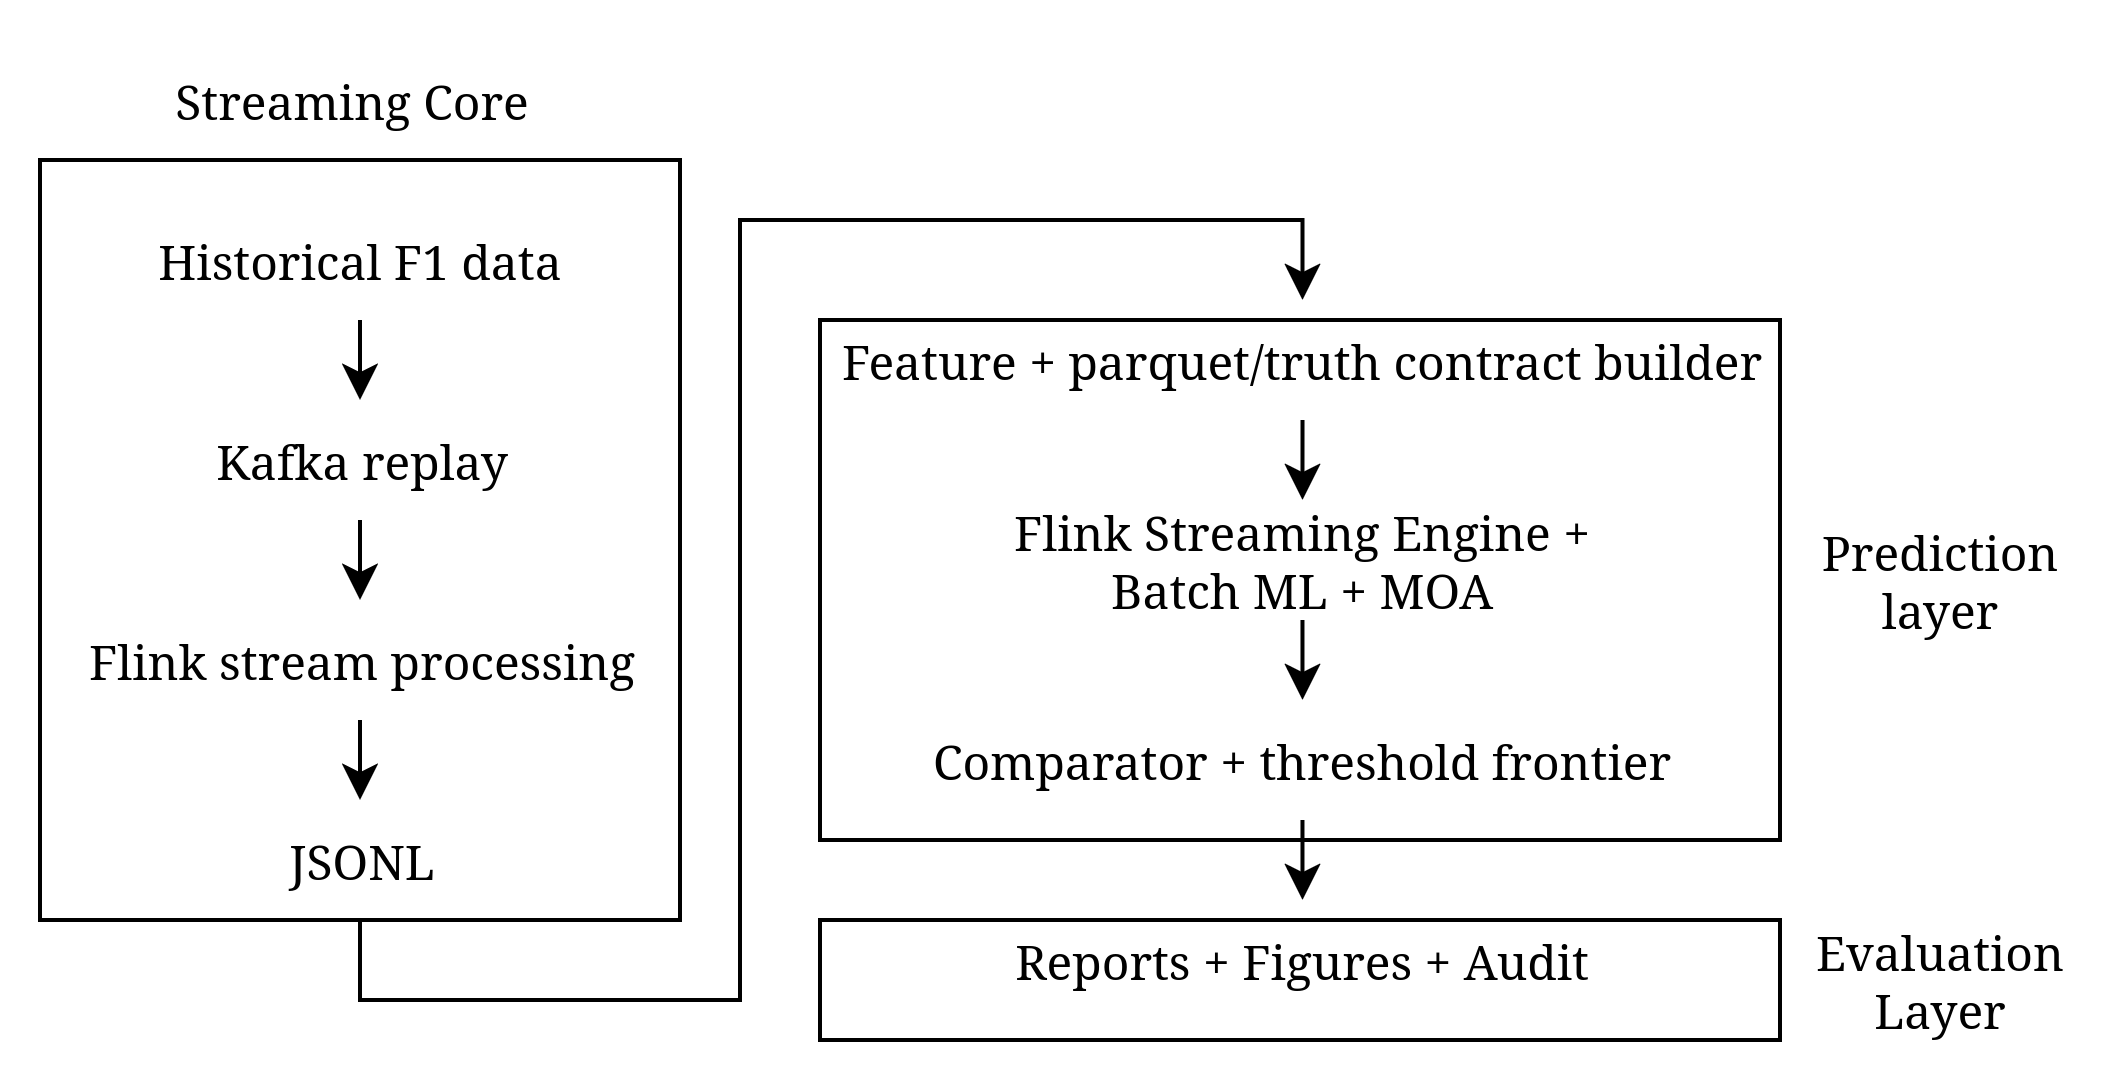
\includegraphics[width=\columnwidth]{Images/ch4/full_architecture.png}
    \caption{Pipeline architecture from historical race extraction to streaming, learning, and comparison.}
    \label{fig:exec_full_architecture}
\end{figure}

The ingestion stage starts from a race preparation script. FastF1 sessions are loaded and converted into a race snapshot containing lap events, telemetry-related observations, track status changes, weather, stint information, pit stop evidence, and race metadata. Lap events are enriched with team and stint data, total laps, pit-loss estimates, and available gap information. Events are then sorted by absolute timestamp and replayed through Kafka topics, so the historical race becomes an ordered log.

The Flink job consumes the replay topics and builds the \textbf{live race context} with \textbf{event-time processing}. Track status is broadcast to the operators that need it, while driver streams are keyed by race and driver. This allows stateful operators to maintain stint-specific and driver-specific information. Windowed computations group cars by race and lap to identify rivals ahead and behind, compute relevant gaps, and emit machine-learning feature rows as side outputs.

The stateful strategy logic produces several interpretable artifacts:
\begin{itemize}
    \item a tyre drop detector, which keeps the best lap in the current stint and counts consecutive slow laps;
    \item a drop-zone evaluator, which estimates where the driver would rejoin after a pit stop;
    \item a pit stop evaluator, which labels real pit outcomes from post-pit evidence;
    \item a pit suggestion stream, which scores whether the current context supports MONITOR, GOOD\_PIT, or PIT\_NOW.
\end{itemize}

The \textbf{Flink Strategy Engine} is the deterministic baseline. Its score combines pace loss, track status, traffic, strategic pressure, actionability, timing, end-of-race effects, competitive advantage, and uncertainty penalties. The final profile used in the evaluation is a guarded variant: rival pressure can increase urgency, but only when timing, gap, and traffic conditions support the call.

The \textbf{Batch path} uses the same artifacts to build supervised learning matrices for XGBoost. The matrix builder removes leakage-prone columns such as target labels, matched pit evidence, truth-lens flags, eligibility indicators, and metadata. Two feature profiles are compared: No-Year, which removes \texttt{source\_year} after it was identified as a shortcut risk, and Percent, which emphasises race-relative quantities such as race progress and lap-time ratios.

The \textbf{online path} exports the shared matrix logic to ARFF and evaluates MOA learners prequentially. Each instance is first scored, then used for training. The Java vote logger records labels, hard predictions, class votes, and a positive score derived from the vote distribution. These outputs are reconstructed with metadata so that MOA can be compared with Batch and Flink under the same threshold and event-matching logic.

A substantial part of the design is devoted to \textbf{fairness corrections}. The comparator aligns systems on the same race-driver universe, applies the same horizon, distinguishes raw and clean truth lenses, and evaluates both row-level and event-level behaviour. This prevents an implementation detail, such as missing outputs for one driver or a different denominator, from becoming a misleading performance gain.


\section{Experimental Evaluation}
\label{sec:evaluation}
The frozen evaluation uses \textbf{Formula 1 races from 2022 to 2025}, the \texttt{canonical\_sde\_truth} universe, the \texttt{clean\_actionable} lens, horizon $H=2$, and five systems: the Flink Strategy Engine, Batch No-Year, Batch Percent, MOA No-Year, and MOA Percent. Batch systems are evaluated with race-sequential out-of-fold predictions. MOA systems are evaluated prequentially. Flink is evaluated through the persisted pit suggestion stream.

\begin{figure*}[t]
    \centering
    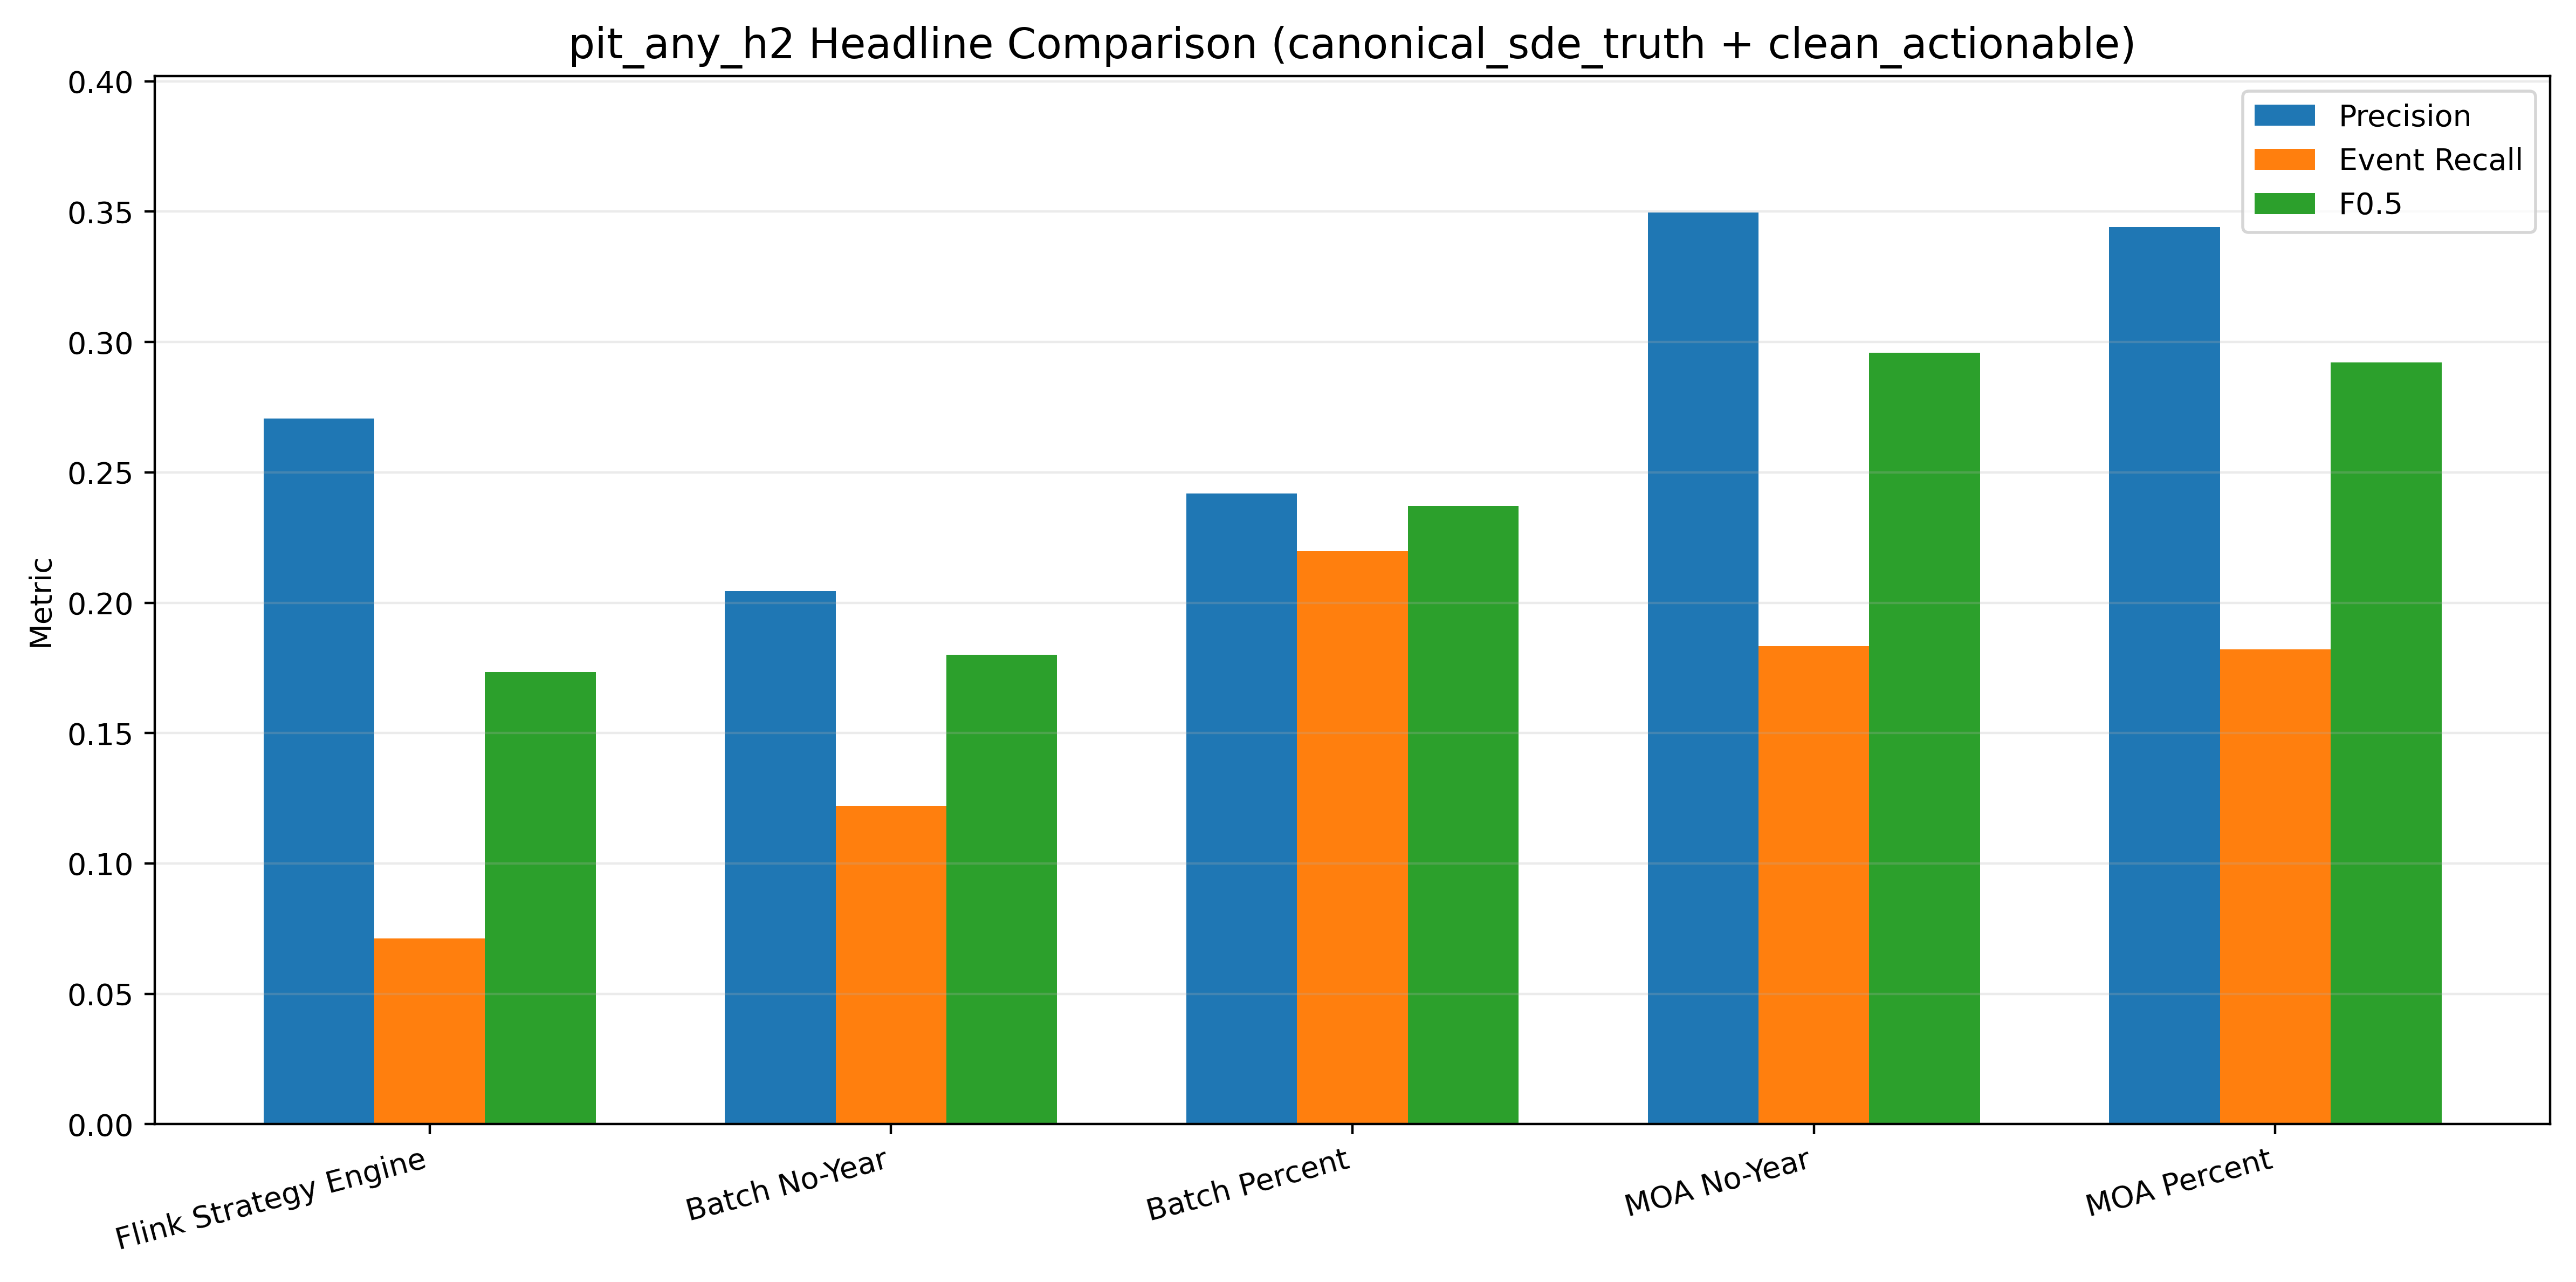
\includegraphics[width=0.48\textwidth]{Images/ch5/pit_any_headline_comparison.png}\hfill
    
\includegraphics[width=0.48\textwidth]{Images/ch5/pit_success_apples_to_apples_main.png}
    \caption{Headline comparison for \texttt{pit\_any\_h2} (left) and strict \texttt{pit\_success\_h2} (right) under the clean actionable protocol.}
    \label{fig:exec_headline_results}
\end{figure*}

For \texttt{pit\_any\_h2}, the learner matrix contains 93,623 driver-lap rows, of which 5,855 are positive, about 6.3\%. The shared comparator event universe contains 3,048 unique eligible pit events. The selected operating points show that \textbf{near-term pit timing is learnable}:
\begin{itemize}
    \item Flink reaches precision 0.271, event coverage 0.071, and $F_{0.5}=0.173$.
    \item Batch Percent reaches the largest coverage, 0.220, with precision 0.242.
    \item MOA No-Year and MOA Percent provide the strongest precision-oriented balance, with precision around 0.35 and $F_{0.5}$ close to 0.30.
\end{itemize}
The precision-recall analysis supports the same conclusion. Average precision for \texttt{pit\_any\_h2} is 0.131 for Batch No-Year, 0.190 for Batch Percent, 0.161 for MOA No-Year, and 0.195 for MOA Percent. The \textbf{Percent feature profile} therefore improves ranking quality for the timing task, especially by replacing absolute or identity-like variables with race-relative signals.

For \texttt{pit\_success\_h2}, the results are more limited and more informative. The \textbf{strict contract} counts unmatched positive calls and failed matched pits as false positives. Under this rule:
\begin{itemize}
    \item Flink PIT\_NOW obtains strict precision 0.080, coverage 0.083, and $F_{0.5}=0.081$.
    \item \textbf{MOA Percent} is the strongest selected system, with precision 0.365, coverage 0.029, and $F_{0.5}=0.111$.
    \item relaxed thresholds can recover more successful events, but only by accepting more false positives.
\end{itemize}
A relaxed MOA Percent point raises success coverage to 0.169 with precision 0.205. Batch Percent under a relaxed threshold reaches coverage 0.083 with precision 0.105. This confirms that successful-pit prediction is sparse and threshold-sensitive.

The Flink diagnostics further clarify why strict precision is necessary. For PIT\_NOW alerts, the matched-pit success rate is 0.583, but strict precision is only 0.080. When GOOD\_PIT alerts are added, the matched-pit success rate increases to 0.628 while strict precision decreases to 0.060. \textbf{Matched-pit success rate} describes only recommendations that eventually match a real pit stop; it ignores recommendations that never match any pit evidence.

Runtime measurements show the expected engineering trade-off. Batch No-Year requires about 1 minute and 44 seconds for \texttt{pit\_any\_h2} and 1 minute and 41 seconds for \texttt{pit\_success\_h2}; Batch Percent is slightly faster. MOA runs in a single pass and requires about 18--24 seconds for the target/profile combinations.

Race-level Kappa and G-Mean provide a view of stability across events. For \texttt{pit\_any\_h2}, Batch Percent and MOA produce more consistent positive behaviour than the deterministic baseline, although results still oscillate by race. For \texttt{pit\_success\_h2}, the support is smaller and race-level metrics are noisier.

Finally, explainability is treated differently for each system. Flink is transparent by construction because its score components and gates are explicit. Batch XGBoost is analysed with SHAP, which confirms the importance of race-context variables and supports the removal of shortcut features. MOA scores are vote-derived ranking scores rather than calibrated probabilities, and faithful online explanations are not retained in the final protocol.


\section{Conclusions}
\label{sec:conclusions}
The thesis shows that pit stop decision support can be studied from historical Formula 1 data only if the problem is made 
\textbf{temporal, contractual, and comparable}. Historical records must be replayed or reconstructed in event order; the target must state exactly 
what a correct positive recommendation means; and systems must be evaluated on the same truth universe. Without these constraints, the comparison 
between a rule engine, a Batch learner, and an online learner would mix modelling quality with leakage, denominator differences, or post-race information.

The first research question receives a positive answer. Near-term pit timing, represented by \textbf{\texttt{pit\_any\_h2}}, is a \textbf{learnable task}. 
The learning systems improve over the deterministic baseline, with Batch Percent providing the largest event coverage and MOA offering the 
best precision-oriented operating points. The result shows that pit stops can't be predicted perfectly, but race state patterns contain 
enough information to support better than rule-baseline timing recommendations under a live like chronology.

The second research question receives a more cautious answer. Successful pit recommendation, represented by \textbf{\texttt{pit\_success\_h2}}, 
is \textbf{much harder}. MOA Percent obtains the cleanest selected strict operating point, but coverage remains low. Relaxed thresholds can recover
more events, at the cost of more false positives. This confirms that successful pit prediction is harder than pit timing: 
it depends on later race development, rival reactions, traffic, tyre performance, and the imperfect heuristic used to classify pit outcomes.

The main limitations follow from the experimental nature of the work. The replay is controlled and reproducible, but it is not a production live 
feed with all latency, correction, missing-data, and failure modes. The PitStopEvaluator is a useful approximation of outcome quality, not yet a full 
strategic utility model. Success labels are sparse, so race-level diagnostics can be unstable. Thresholds strongly influence the apparent behaviour of 
each system. Finally, only a limited set of learners is evaluated: XGBoost for Batch learning and OzaBoostADWIN for MOA online learning.

Future work should therefore move in four directions. First, the pipeline should be connected to a live ingestion setting, so that delay and 
missing-data behaviour can be evaluated directly. Second, the truth model should be refined through richer outcome definitions, probabilistic labels, 
or expert validation. Third, the learning problem could move from row-level classification toward event-level ranking, time-to-pit modelling, or 
sequence-aware policies under a fixed false-positive budget. Fourth, online learning should be expanded with stronger calibration and faithful 
online explainability.

Overall, the contribution of the thesis is an \textbf{executable and auditable framework} for asking a precise question: when a system says ``pit now'', 
what contract is it satisfying, what information was available, and how should that call be counted? The answer is strongest for pit timing and still 
preliminary for successful pit recommendation, but the pipeline makes both problems measurable in a reproducible way.


\begingroup
\scriptsize
\setlength{\bibsep}{0pt}
\renewcommand{\refname}{Bibliography}
\bibliography{Thesis_bibliography}
\endgroup

\end{document}
